\chapter{Results}

In this chapter, we present the results for various models on three datasets.\todo{What datasets? Describe or make a reference.} We compare the performance of the models and the datasets. This includes comparison of open source data downloaded from the Internet with the proprietary data provided by the private company. In the third section, we compare the performance for different number of recommendations.\todo{What else? There should probably be more.}

\section{Comparison of Models}

In the following text, comparison of the models is presented. We show the accuracy, precision and recall of these models on three datasets.\todo{What models? Explain or provide reference.}\todo{Explanation of these measurement metrics should be somewhere and perhaps a reference would be in order.} This comparison allows us to conclude what model is best for this application.

\subsection{Firefox Data}

On Figure~\ref{fig:results.models.firefox}, you can see the performance of the chosen models on Firefox data. The SVM model with TF-IDF weighing achieves the best performance with accuracy of 57\%. It's precision and recall also outperforms all the other approaches with values of 51\% and 45\%. The same model with LSI takes second place. The only model other than SVM that approaches SVM with it's performance is CART, especially with TF-IDF weighing.

\begin{figure}[htbp]
    \centering
        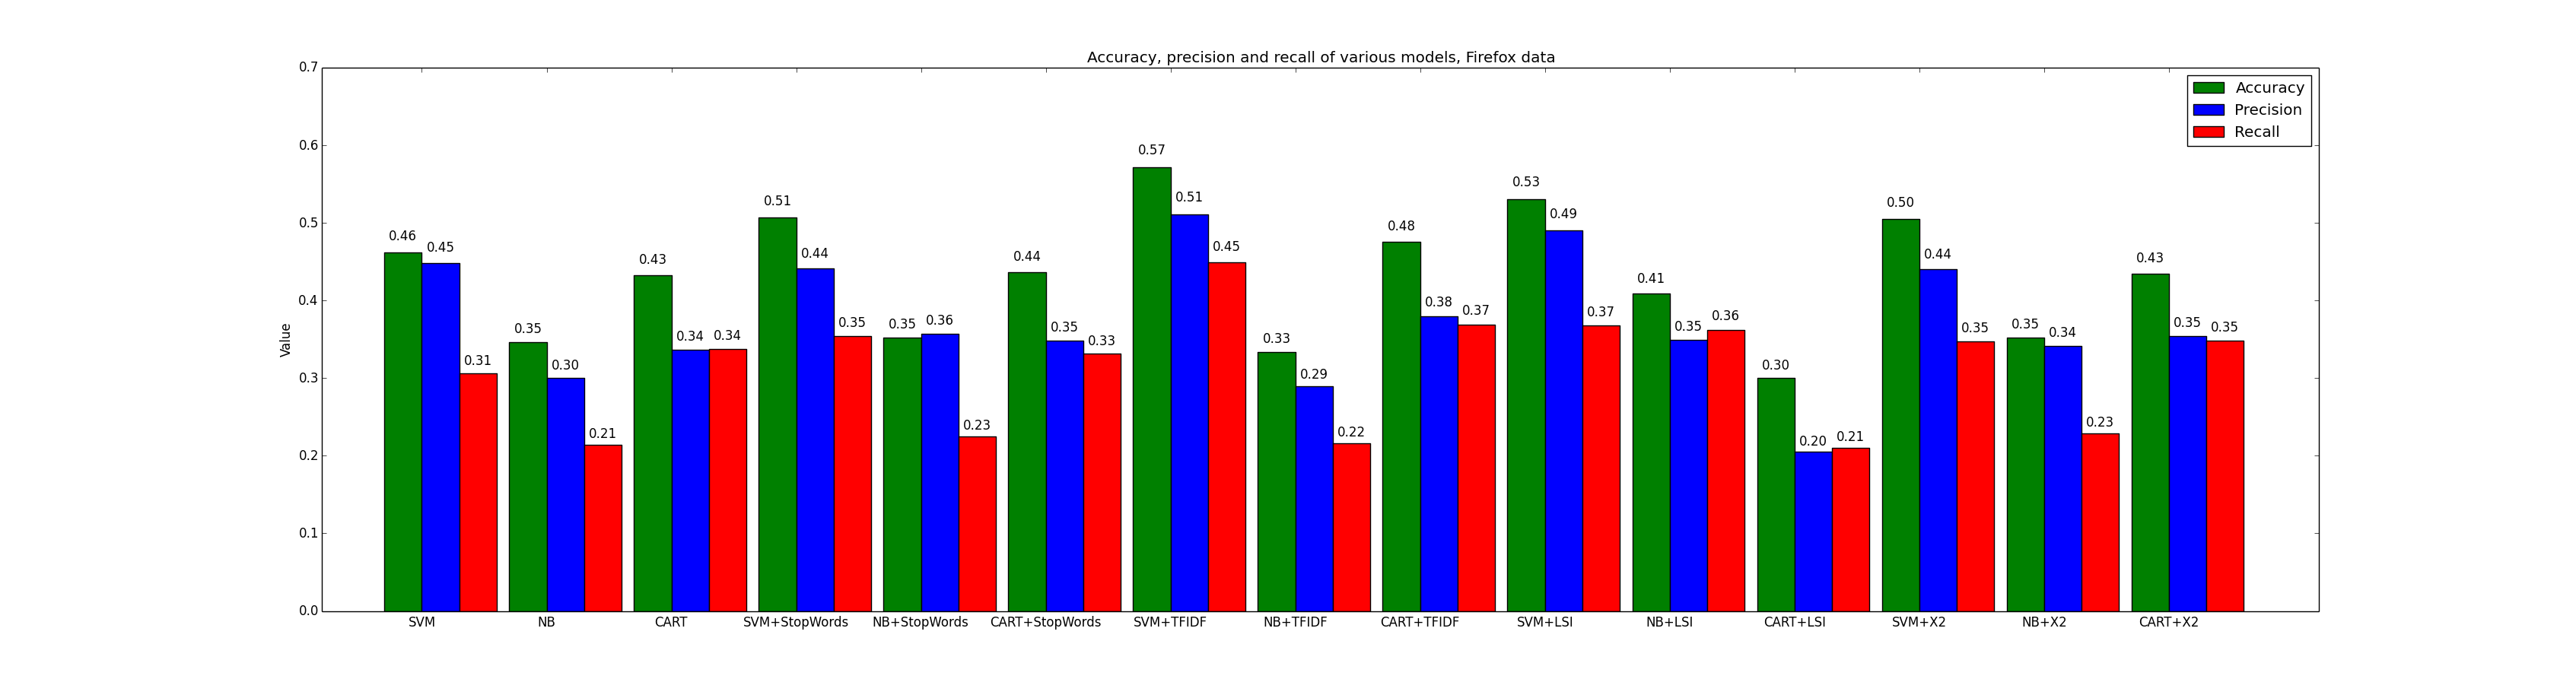
\includegraphics[width=\textwidth,trim=8cm 1cm 8cm 1cm,clip]{./images/comparison_of_models/firefox.png}
    \caption{Comparison of models on Firefox data.}
    \label{fig:results.models.firefox}
\end{figure}

\subsection{Netbeans Data}

The performance of the models on Netbeans data is shown on Figure~\ref{fig:results.models.netbeans}. It is clear that the SVM model with TF-IDF weighing performs best even on the Netbeans data, although in this case the LSI feature extraction technique does not seem to perform as well as in the previous case. The accuracy, precision and recall of the approach are 53\%, 53\% and 49\% respectively. Sole SVM model and SVM+$\chi^2$ model perform similarly as far as precision is concerned, while the accuracy and recall values are lagging behind by a considerable margin. None of the other models offer better performance than even sole SVM model on this data, which suggests that SVM is a very good choice in this domain.

\begin{figure}[htbp]
    \centering
        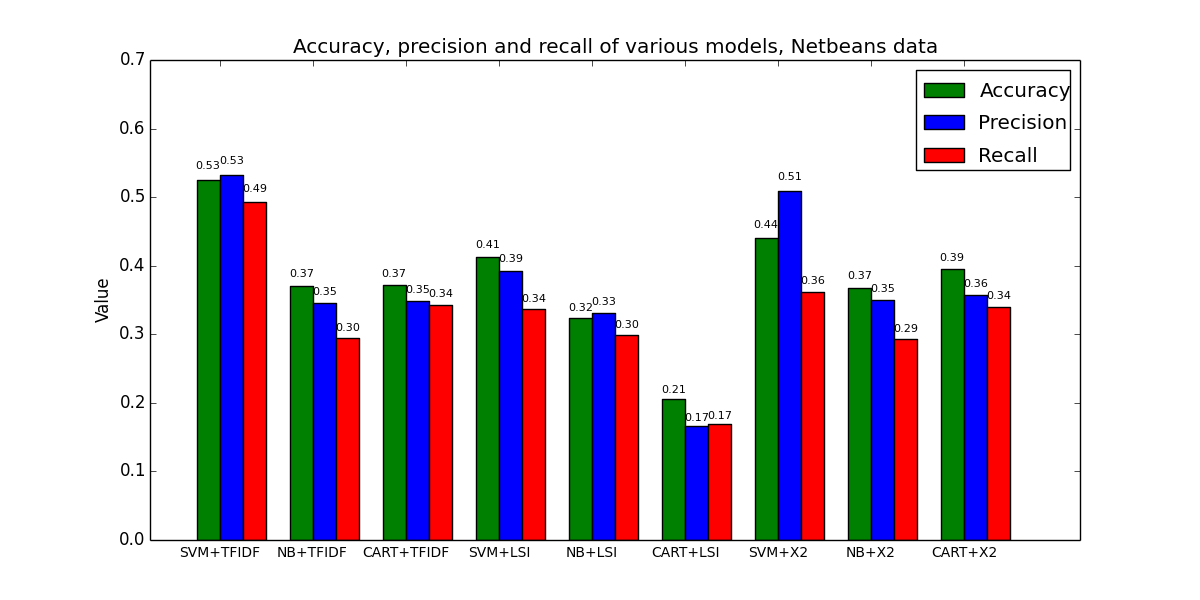
\includegraphics[width=\textwidth,trim=8cm 1cm 8cm 1cm,clip]{./images/comparison_of_models/netbeans.png}
    \caption{Comparison of models on Netbeans data.}
    \label{fig:results.models.netbeans}
\end{figure}

\subsection{Proprietary Data}

In this case, the performance of all models decreased a lot in comparison with the other datasets. However, even in this case, the SVM model with TF-IDF offers the best performance of 37\% accuracy, 32\% precision and 31\% recall. The same model with LSI also shows quite a good performance and quite surprisingly, the Naive Bayes model with LSI performs quite well as far as precision and recall is concerned. Figure~\ref{fig:results.models.proprietary} presents the results in graphical manner.

\begin{figure}[htbp]
    \centering
        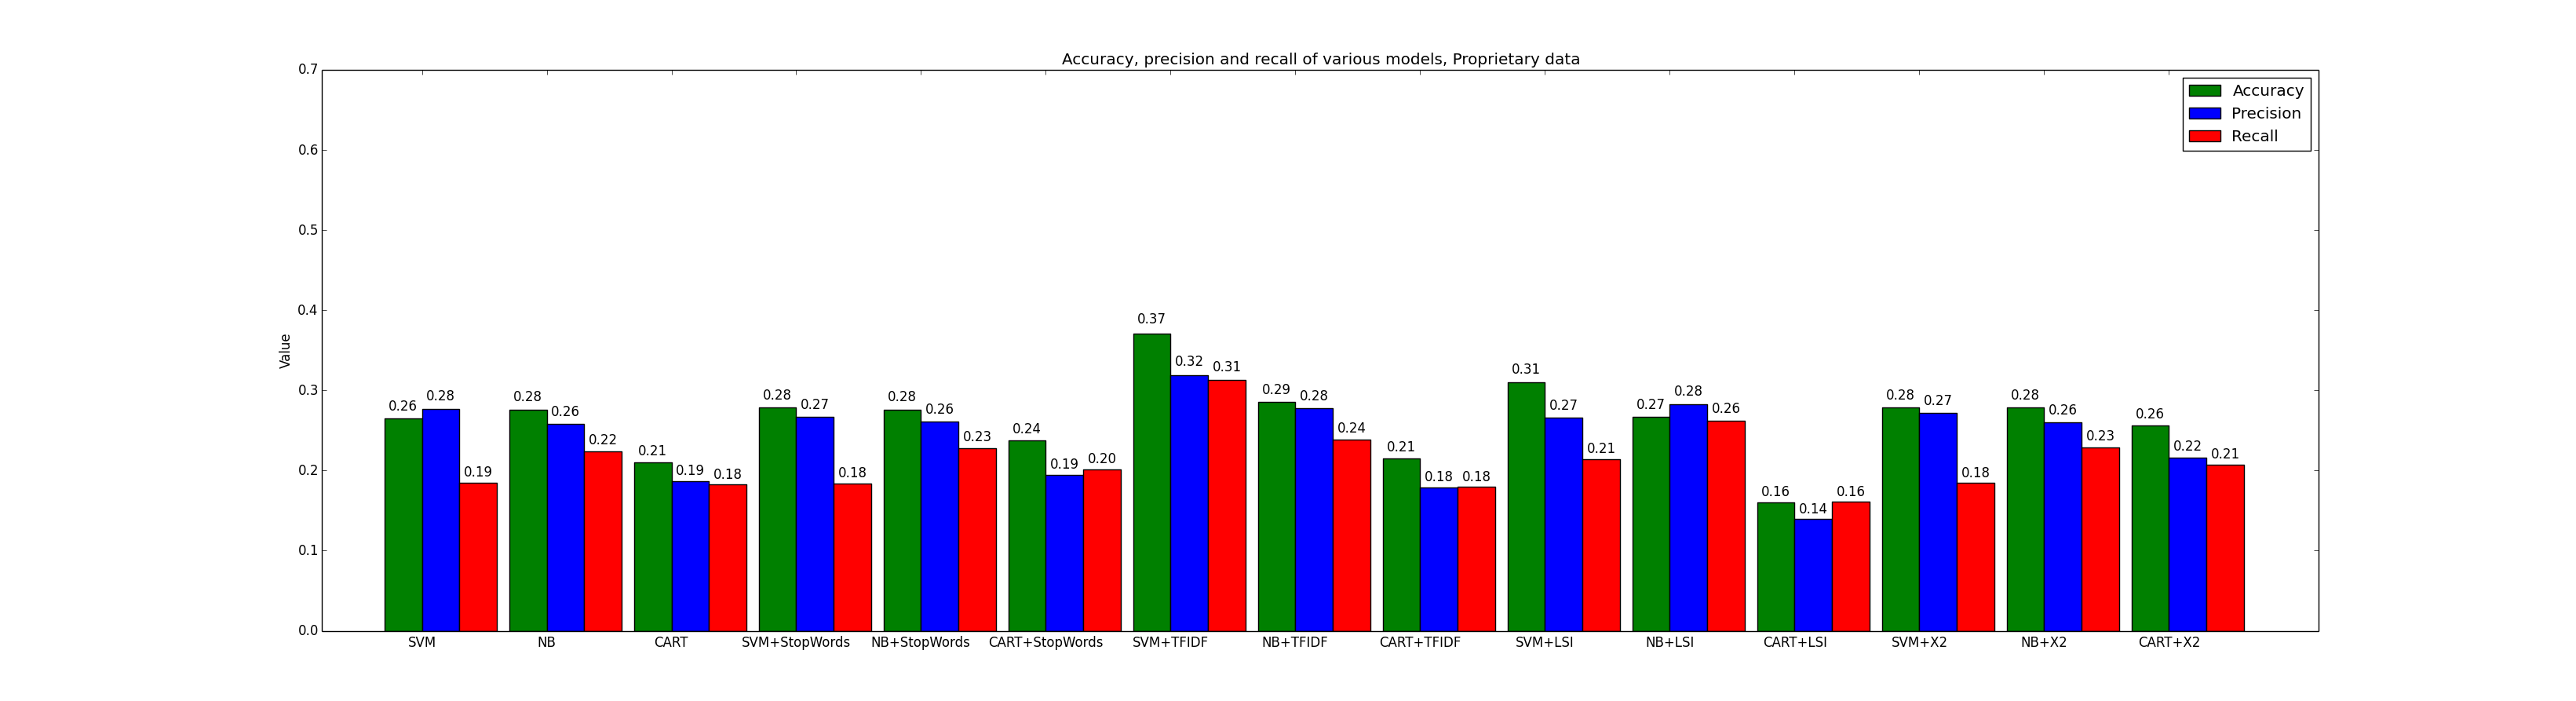
\includegraphics[width=\textwidth,trim=8cm 1cm 8cm 1cm,clip]{./images/comparison_of_models/proprietary.png}
    \caption{Comparison of models on the Proprietary data.}
    \label{fig:results.models.proprietary}
\end{figure}

\subsection{Conclusion}

The comparison shows that SVM with TF-IDF weighing performs best on all datasets. Not only that, it also generalizes very well, because there was no need to readjust the parameters of the model to get the best or nearly the best performance for all datasets. The disadvantage of the model is that it is the most computationally complex one, because SVM is the slowest of the three models, there are a lot of classes and there are a lot of features. This can be at least partially dealt with by using $\chi^2$ feature extraction in conjunction with TF-IDF while sacrificing some of the performance.

\section{Comparison of Datasets}

The main purpose of this section is to compare proprietary dataset with open-source dataset. The open-source dataset used for this is from the Firefox project. We selected equal number of reports from both datasets to construct an accurate comparison.\todo{Maybe it would be useful to compare with the Netbeans data too.}\todo{And also it could be quite interesting to use the CART model too.}

\subsection{Naive Bayes Model}

The first model for comparison is Naive Bayes. The only used feature extraction method for this model is stop-words removal.

First plot (Figure \ref{fig:results.datasets.nb_accuracy}) represents accuracy of the Naive Bayes model. You can already see that the open source data perform better than the proprietary data. Accuracy of the classifier is 35 \% vs 24 \% when $x$ (see above) is set to 30. In the following text, we will always compare the results of this setting of parameter $x$ as we believe that is the best production value for the given size of the dataset.

\begin{figure}[htbp]
    \centering
        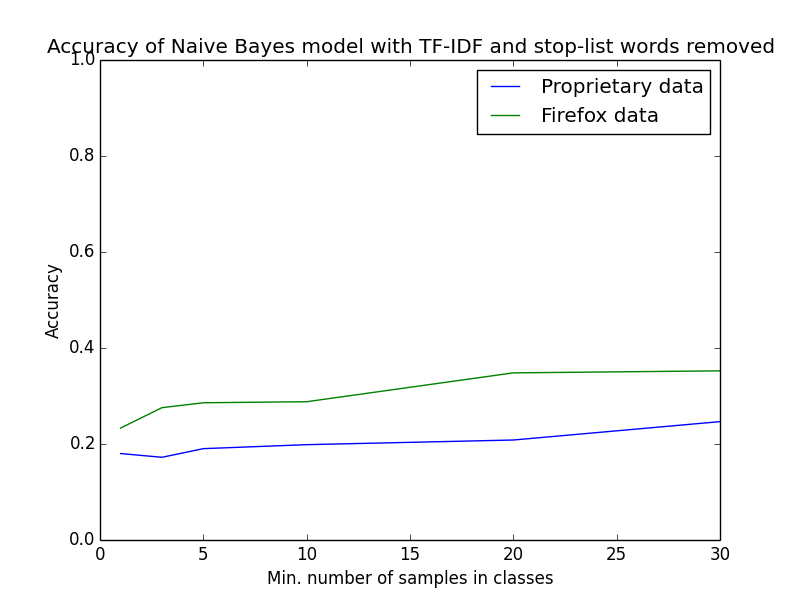
\includegraphics[width=250px]{./images/prop_vs_os/nb_accuracy.png}
    \caption{Comparison of accuracy of Naive Bayes model.}
    \label{fig:results.datasets.nb_accuracy}
\end{figure}

Second plot (Figure \ref{fig:results.datasets.nb_precision}) is a representation of precision of the same model. Precision of the classifier is 46 \% and 22 \% for the open source and proprietary data, respectively.

\begin{figure}[htbp]
    \centering
        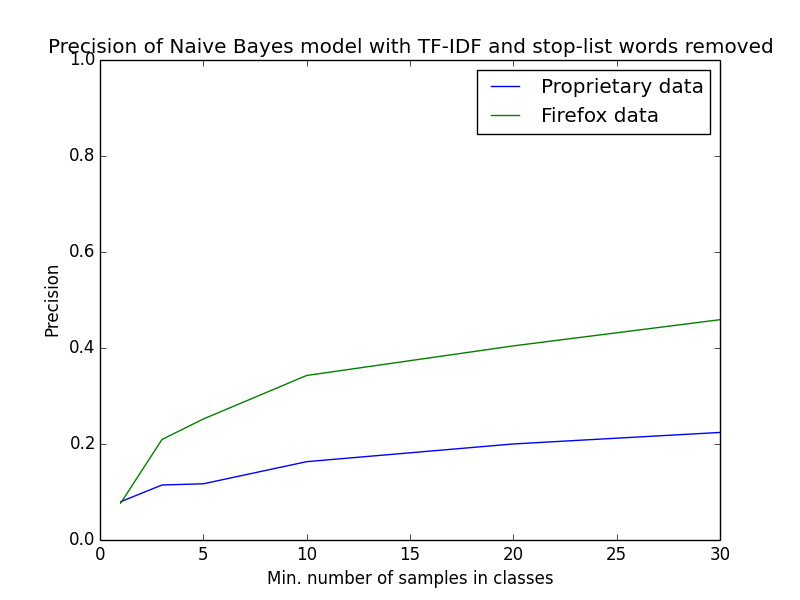
\includegraphics[width=250px]{./images/prop_vs_os/nb_precision.png}
    \caption{Comparison of precision of Naive Bayes model.}
    \label{fig:results.datasets.nb_precision}
\end{figure}

Figure \ref{fig:results.datasets.nb_recall} shows recall of the Naive Bayes model. Recall value is 29 \% for the open source data and 19 \% for the proprietary data.

\begin{figure}[htbp]
    \centering
        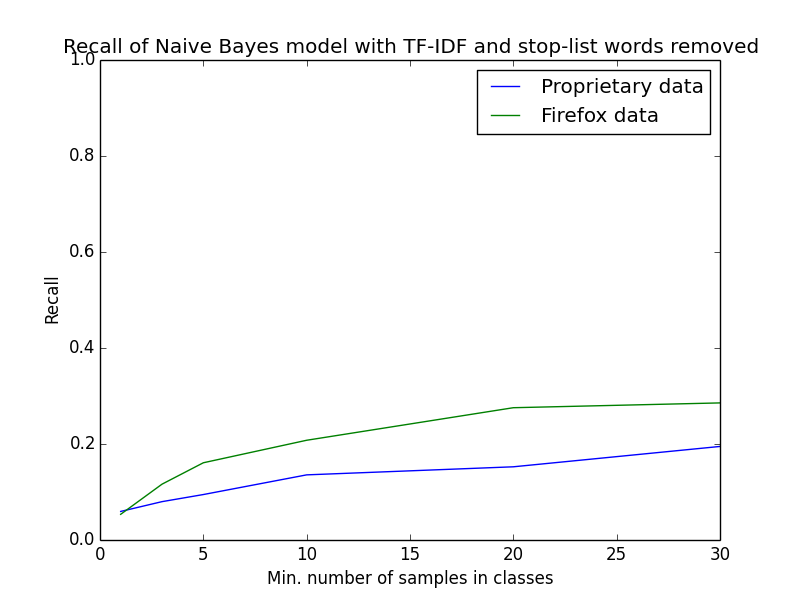
\includegraphics[width=250px]{./images/prop_vs_os/nb_recall.png}
    \caption{Comparison of recall of Naive Bayes model.}
    \label{fig:results.datasets.nb_recall}
\end{figure}

\subsection{Support Vector Machine Model}

The second model used for comparison of the proprietary dataset with the open-source dataset is Support Vector Machine model with TF-IDF weighing and stop-words removal as this model shows the most promising results.

Figure \ref{fig:results.datasets.svm_accuracy} visualizes accuracy of the model. Even with this model, the open source data perform much better with accuracy value of 54 \% vs 33 \% of the proprietary data.

\begin{figure}[htbp]
    \centering
        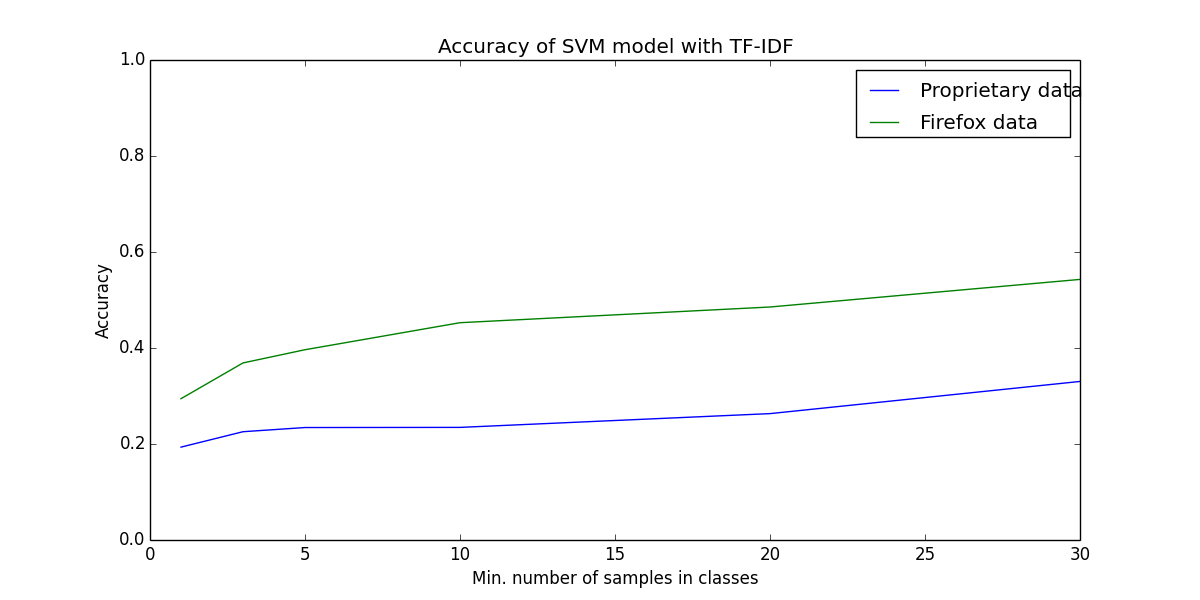
\includegraphics[width=250px]{./images/prop_vs_os/svm_accuracy.png}
    \caption{Comparison of accuracy of SVM model.}
    \label{fig:results.datasets.svm_accuracy}
\end{figure}

Precision of the SVM model is pictured on figure \ref{fig:results.datasets.svm_precision}. It again clearly shows that the precision value of the open source data is higher (again about 54 \%) than the precision value of the proprietary data (32 \%).

\begin{figure}[htbp]
    \centering
        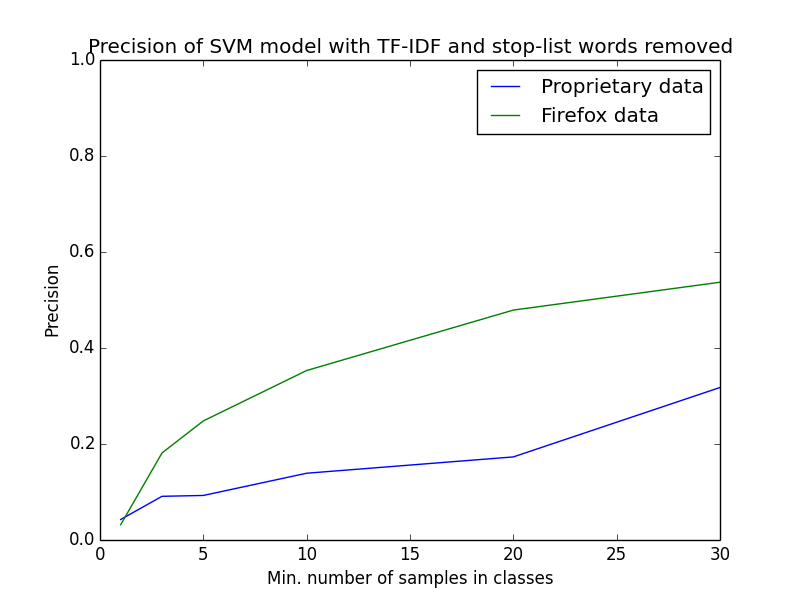
\includegraphics[width=250px]{./images/prop_vs_os/svm_precision.png}
    \caption{Comparison of precision of SVM model.}
    \label{fig:results.datasets.svm_precision}
\end{figure}

Last plot (Figure \ref{fig:results.datasets.svm_recall}) shows the recall of the same model. On the open source data, the classifier achieved recall value of 49 \% and on the proprietary data 26 \%.

\begin{figure}[htbp]
    \centering
        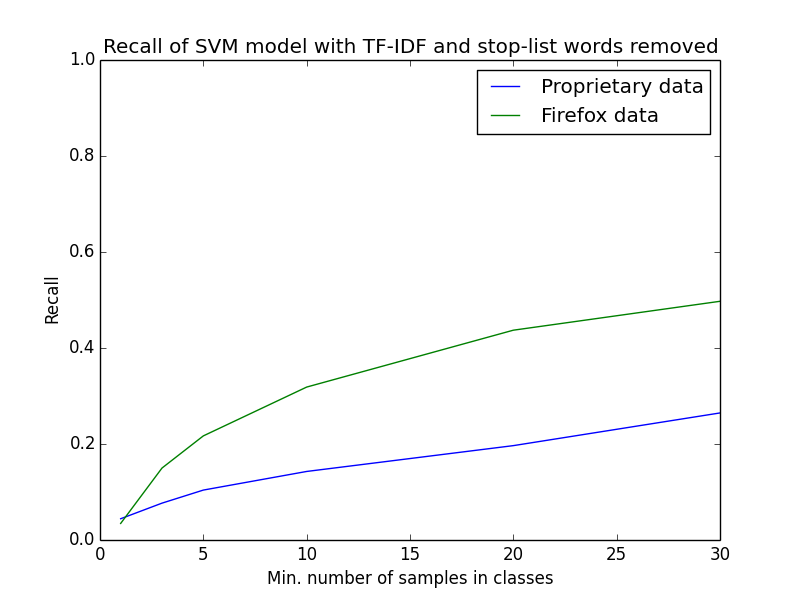
\includegraphics[width=250px]{./images/prop_vs_os/svm_recall.png}
    \caption{Comparison of recall of SVM model.}
    \label{fig:results.datasets.svm_recall}
\end{figure}

\subsection{Conclusion}

The results clearly show that the open-source data provide much better performance. The number of classes is very similar and the number of reports used for training too, so it is clear that the quality of the open-source reports is higher.\todo{Or maybe there is something else? Try to figure out if that is really the case, if it is, it might be better to provide a better explanation.}

\section{Comparison of Performance for Variable Number of Recommendations}

We look at the performance of the models for different number of recommendations in this section. The plots will show the performance for number of recommendations from 1 to 10.\todo{More than one model might be in order.}

\subsection{Support Vector Machine Model}

For this comparison, we, again, take the SVM model with TF-IDF weighing and stop-words removed. Figure \ref{fig:results.topx.svm_accuracy} shows how the accuracy increases when the number of recommendations increases, which is expected as the more there are recommendation, the higher the chance of a hit is.\todo{Precision and recall would be useful too maybe.}

\begin{figure}[htbp]
    \centering
        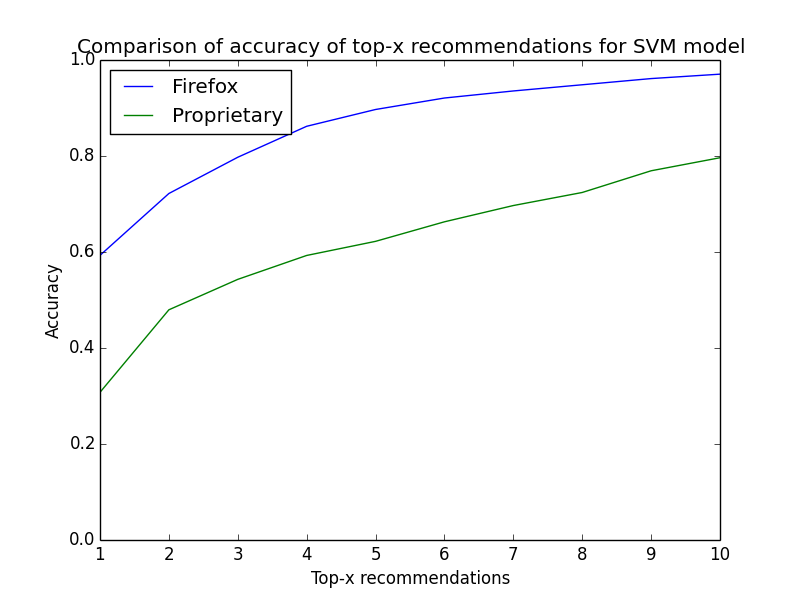
\includegraphics[width=250px]{./images/top_x_comparison/svm_accuracy.png}
    \caption{Comparison of accuracy of top-x recommendations for SVM model.}
    \label{fig:results.topx.svm_accuracy}
\end{figure}

It is apparent from the plot that the highest performance boost happens when the number of recommendations changes from one to two both for the proprietary data and the Firefox data. 

\subsection{Conclusion}

From the results in this section, we concluded that the best number of recommendations to suggest to users is 5. The performance does not increase very much with more recommendations and it would probably only lead to confusion if the number of recommendations was too high.